\tikzset{every picture/.style={line width=0.75pt}} %set default line width to 0.75pt        
\noindent
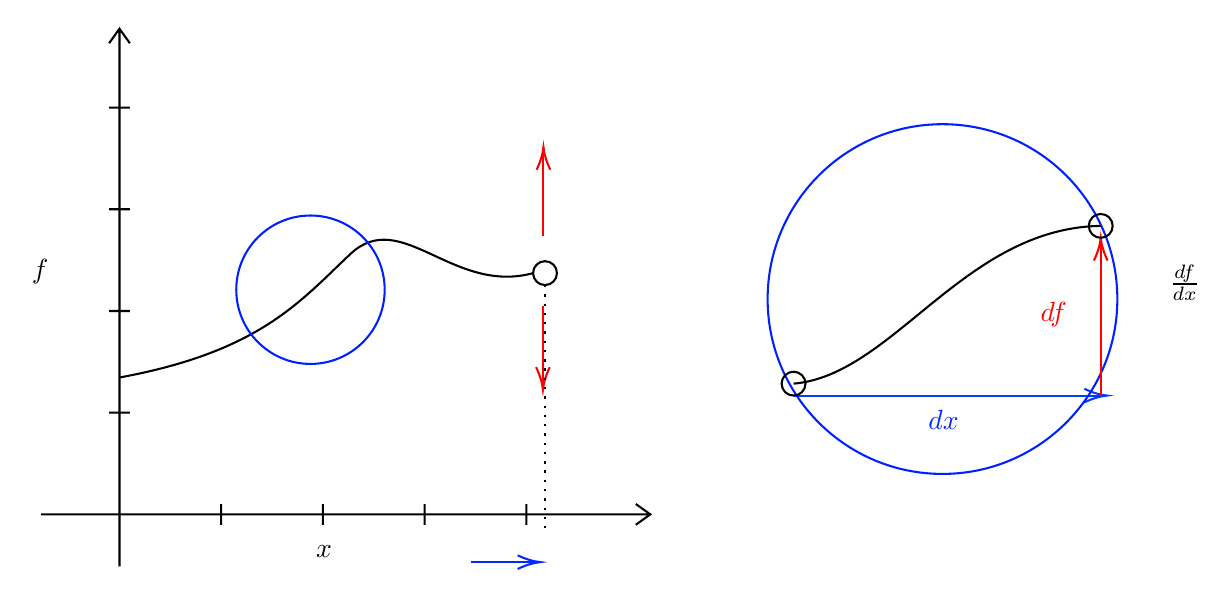
\begin{tikzpicture}[x=0.75pt,y=0.75pt,yscale=-1,xscale=1]
%uncomment if require: \path (0,300); %set diagram left start at 0, and has height of 300

%Shape: Axis 2D [id:dp2705874217955565] 
\draw  (61,251) -- (354.5,251)(98.73,17) -- (98.73,276) (347.5,246) -- (354.5,251) -- (347.5,256) (93.73,24) -- (98.73,17) -- (103.73,24) (147.73,246) -- (147.73,256)(196.73,246) -- (196.73,256)(245.73,246) -- (245.73,256)(294.73,246) -- (294.73,256)(93.73,202) -- (103.73,202)(93.73,153) -- (103.73,153)(93.73,104) -- (103.73,104)(93.73,55) -- (103.73,55) ;
\draw   ;
%Shape: Circle [id:dp5289460412049012] 
\draw   (298,134.75) .. controls (298,131.57) and (300.57,129) .. (303.75,129) .. controls (306.93,129) and (309.5,131.57) .. (309.5,134.75) .. controls (309.5,137.93) and (306.93,140.5) .. (303.75,140.5) .. controls (300.57,140.5) and (298,137.93) .. (298,134.75) -- cycle ;
%Curve Lines [id:da5722046762054834] 
\draw    (99,185) .. controls (166.32,172.54) and (185.62,148.48) .. (210,125.53) .. controls (234.38,102.59) and (259.35,145.33) .. (298,134.75) ;
%Straight Lines [id:da03826940790031441] 
\draw [color={rgb, 255:red, 255; green, 0; blue, 0 }  ,draw opacity=1 ]   (303,117) -- (303,76) ;
\draw [shift={(303,74)}, rotate = 450] [color={rgb, 255:red, 255; green, 0; blue, 0 }  ,draw opacity=1 ][line width=0.75]    (10.93,-3.29) .. controls (6.95,-1.4) and (3.31,-0.3) .. (0,0) .. controls (3.31,0.3) and (6.95,1.4) .. (10.93,3.29)   ;
%Straight Lines [id:da702743188727071] 
\draw [color={rgb, 255:red, 255; green, 0; blue, 0 }  ,draw opacity=1 ]   (302.75,150.5) -- (302.75,189) ;
\draw [shift={(302.75,191)}, rotate = 270] [color={rgb, 255:red, 255; green, 0; blue, 0 }  ,draw opacity=1 ][line width=0.75]    (10.93,-3.29) .. controls (6.95,-1.4) and (3.31,-0.3) .. (0,0) .. controls (3.31,0.3) and (6.95,1.4) .. (10.93,3.29)   ;
%Straight Lines [id:da7155741388130133] 
\draw  [dash pattern={on 0.84pt off 2.51pt}]  (303.75,140.5) -- (303.75,259) ;
%Straight Lines [id:da8882950487937341] 
\draw [color={rgb, 255:red, 0; green, 42; blue, 255 }  ,draw opacity=1 ]   (268,274) -- (299.5,274) ;
\draw [shift={(301.5,274)}, rotate = 180] [color={rgb, 255:red, 0; green, 42; blue, 255 }  ,draw opacity=1 ][line width=0.75]    (10.93,-3.29) .. controls (6.95,-1.4) and (3.31,-0.3) .. (0,0) .. controls (3.31,0.3) and (6.95,1.4) .. (10.93,3.29)   ;
%Shape: Circle [id:dp6966573631790741] 
\draw  [color={rgb, 255:red, 0; green, 33; blue, 255 }  ,draw opacity=1 ] (155,142.75) .. controls (155,123.01) and (171.01,107) .. (190.75,107) .. controls (210.49,107) and (226.5,123.01) .. (226.5,142.75) .. controls (226.5,162.49) and (210.49,178.5) .. (190.75,178.5) .. controls (171.01,178.5) and (155,162.49) .. (155,142.75) -- cycle ;
%Straight Lines [id:da29696501529074004] 
\draw [color={rgb, 255:red, 0; green, 59; blue, 255 }  ,draw opacity=1 ]   (423.5,193.75) -- (572.5,193.75) ;
\draw [shift={(574.5,193.75)}, rotate = 180] [color={rgb, 255:red, 0; green, 59; blue, 255 }  ,draw opacity=1 ][line width=0.75]    (10.93,-3.29) .. controls (6.95,-1.4) and (3.31,-0.3) .. (0,0) .. controls (3.31,0.3) and (6.95,1.4) .. (10.93,3.29)   ;
%Shape: Circle [id:dp3358182818605919] 
\draw  [color={rgb, 255:red, 0; green, 33; blue, 255 }  ,draw opacity=1 ] (411,147.25) .. controls (411,100.72) and (448.72,63) .. (495.25,63) .. controls (541.78,63) and (579.5,100.72) .. (579.5,147.25) .. controls (579.5,193.78) and (541.78,231.5) .. (495.25,231.5) .. controls (448.72,231.5) and (411,193.78) .. (411,147.25) -- cycle ;
%Curve Lines [id:da06927978322565154] 
\draw    (423.5,188) .. controls (471.5,184) and (505.5,113) .. (571.5,112) ;
%Straight Lines [id:da6621083467521226] 
\draw [color={rgb, 255:red, 255; green, 0; blue, 0 }  ,draw opacity=1 ]   (571.5,193.75) -- (571.5,119.75) ;
\draw [shift={(571.5,117.75)}, rotate = 450] [color={rgb, 255:red, 255; green, 0; blue, 0 }  ,draw opacity=1 ][line width=0.75]    (10.93,-3.29) .. controls (6.95,-1.4) and (3.31,-0.3) .. (0,0) .. controls (3.31,0.3) and (6.95,1.4) .. (10.93,3.29)   ;
%Shape: Circle [id:dp07500667711688713] 
\draw   (417.75,188) .. controls (417.75,184.82) and (420.32,182.25) .. (423.5,182.25) .. controls (426.68,182.25) and (429.25,184.82) .. (429.25,188) .. controls (429.25,191.18) and (426.68,193.75) .. (423.5,193.75) .. controls (420.32,193.75) and (417.75,191.18) .. (417.75,188) -- cycle ;
%Shape: Circle [id:dp09749937355008642] 
\draw   (565.75,112) .. controls (565.75,108.82) and (568.32,106.25) .. (571.5,106.25) .. controls (574.68,106.25) and (577.25,108.82) .. (577.25,112) .. controls (577.25,115.18) and (574.68,117.75) .. (571.5,117.75) .. controls (568.32,117.75) and (565.75,115.18) .. (565.75,112) -- cycle ;

% Text Node
\draw (55,126.4) node [anchor=north west][inner sep=0.75pt]    {$f$};
% Text Node
\draw (192,264.4) node [anchor=north west][inner sep=0.75pt]    {$x$};
% Text Node
\draw (541,147.4) node [anchor=north west][inner sep=0.75pt]  [color={rgb, 255:red, 255; green, 0; blue, 0 }  ,opacity=1 ]  {$df$};
% Text Node
\draw (487,199.4) node [anchor=north west][inner sep=0.75pt]  [color={rgb, 255:red, 0; green, 42; blue, 255 }  ,opacity=1 ]  {$dx$};
% Text Node
\draw (603,129.4) node [anchor=north west][inner sep=0.75pt]    {$\frac{df}{dx}$};


\end{tikzpicture}